
\chapter{PROGRESSION OF CONTROL SYSTEM SOFTWARE}
\label{chap:ProgressionOfControlSystemSoftware}

This research spans five major rewrites of the ADCS software.  This chapter covers the improvements made through the first four versions.  The final TSatPy version of the software that is used throughout this thesis is covered in greater detail in Chapter \ref{chap:TSatPy}.  The first four versions covered in Sections \ref{sec:NSSModel} through \ref{sec:ObjectOrientedNSSControlSystem} are written for use with a Numerical Simulation Software (NSS like MATLAB Simulink or Octave).  Section \ref{sec:NSSModel} is a version based upon the work of Vess' ``open-loop'' controller \cite{vessthesis}.  Section \ref{sec:TSatMessageCenter} covers the creation of the ``TSat Message Center'' for sending and receiving control and sensor data.  The ``run-time'' version in Section \ref{sec:RuntimeControlandAnalysis} focuses on better insight into the system behavior through representative visualizations.  Finally, Section \ref{sec:ObjectOrientedNSSControlSystem} covers the object oriented NSS code that merges state data with the functions governing its use.

\section{Numerical Simulation Software Model}
\label{sec:NSSModel}

The work of Vess \cite{vessthesis} includes an ``open loop'' and ``closed loop'' controller.  In the ``open loop'' design, sensor data is transmitted from the TableSat to a laptop where it is used to update a control law via a numerical simulation software package.  The controller calculates the actuator command voltages and sends them back from the laptop to the TableSat.  Vess ultimately abandoned this method for a ``closed loop'' design after encountering too many issues with its reliability.  Figure \ref{fig:TSatSimulinkSendMessageModel} shown the initial NSS model for testing interactions with the UNH NASA MMS TableSat IA where fans are commanded to run with a  12V input and sensor data messages are monitored for yaw measurements.  This version runs into the same issue as Vess' ``open loop'' control where the unreliable UDP communication often causes the model to update at irregular and large intervals.  There are other disadvantages.  For one, it is difficult to navigate the model as it builds in complexity.  There is no ``built-in'' method for ensuring consistency in its operations between edits such as unit testing.  And, any significant insight into the system's behavior can only be obtained after the post processing of data.

Figure \ref{fig:TSatSimulinkSendMessageModel} shows the first test configuration where a twelve volt signal is sent to TableSat IA at the start of the simulation then sensor voltages are received via UPD and the coarse sun sensors are used to calculate the yaw measurement.

\begin{figure}[ht]
  \centerline{\psfig{file=figures/TSatSimulinkSendMessage.eps,width=5.75in}}
  \caption{TSat Send Message Model}
  \label{fig:TSatSimulinkSendMessageModel}
\end{figure}

\section{TSat Message Center}
\label{sec:TSatMessageCenter}

Following deficiencies in the NSS model design, the ``TSat Message Center'' provides direct control of the messages being sent and received through the User Datagram Protocol (UDP) which bypasses the issues of transferring data into and from the NSS model.  Figure \ref{fig:TSatMessageCenter} shows the interface developed for this version of the ADCS that gives direct control of the TableSat.  Users can enable sensor polling that asks for and displays sensor readings at regular intervals.  Users can also manually set fan input voltage commands and interact with the on-board sensor log.  A PID spin rate control regularly checks for incoming sensor data, calculates actuator command voltages and relays this information to the TableSat.
\begin{figure}[ht]
  \centerline{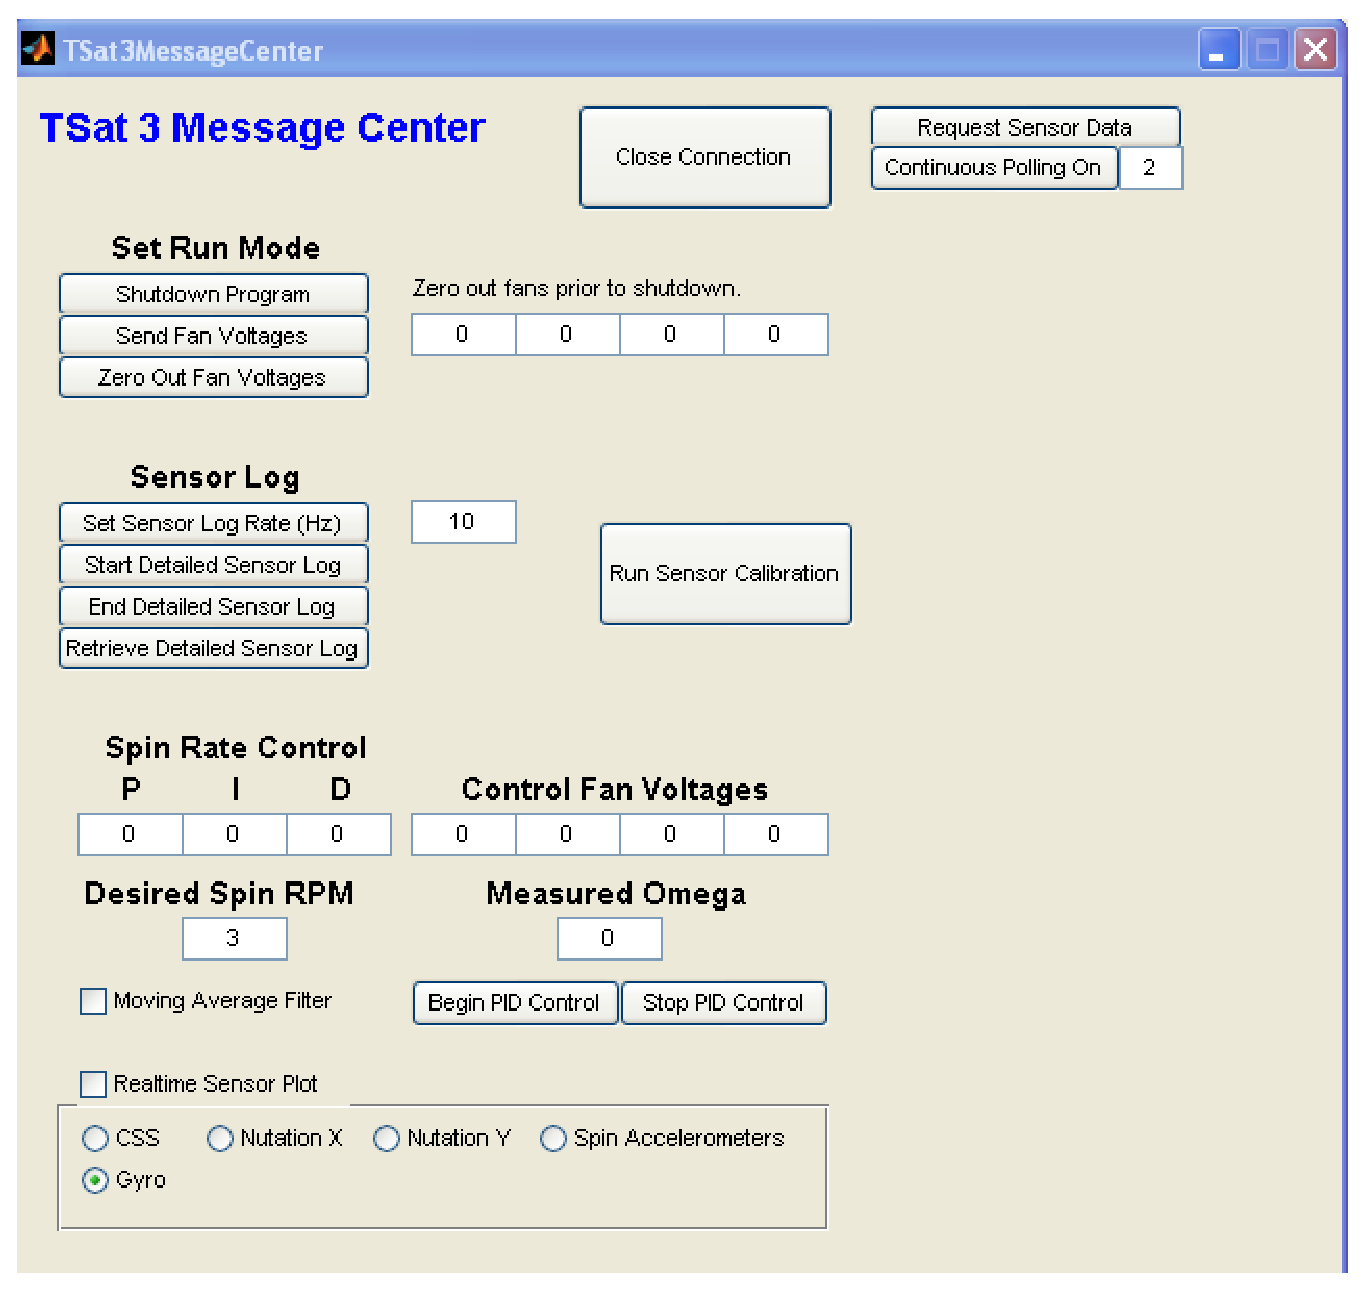
\psfig{file=figures/tsat_message_center.eps,width=5.75in}}
  \caption{TSat Message Center}
  \label{fig:TSatMessageCenter}
\end{figure}

The issue arises when multiple portions of the controller require sensor data, such as during the polling of the sensors while a PID controller is running.  This desired functionality allows for some basic insight into the operation of the TableSat without waiting for the completion of a test.  However, in this case only one feature receives the updates, thus, either leaving TableSat uncontrolled or removing user visibility.  Other issues include having difficulty maintaining the active state of the system in memory since data is not easily shared between functions and having a ballooning code base that requires a dedicated m-file for each new algorithm or function.

At the bottom of Figure \ref{fig:TSatMessageCenter} is a section labeled ``Realtime Sensor Plot''.  This feature is a product of the end of this first version's development cycle but provides the basis for dynamic plotting in later versions.  Persistent variables inside the function remember data submitted which allows it to give a time series view into sensor data or yaw calculations as the experiment runs.  Figure \ref{fig:SimpleRealtime} shows a time lapse of the code in Snippet \ref{code:samplerealtimeplot}.  The plot refreshes in real-time by updating the data behind the sinusoidal plot instead of needing to close and redraw the entire plot which is time intensive especially when the data provided is used to create complex renderings such as is possible in later revisions (Figure \label{fig:RuntimeSatelliteVisualization}).

\begin{listing}[H]
\begin{singlespace}
  \begin{minted}[mathescape,linenos,numbersep=10pt,frame=lines,framesep=2mm]{matlab}
Plot_Realtime(0, 1)
for i = 1:200
    Plot_Realtime(sin(i/20), 0)
end
  \end{minted}
\caption{Create a sample realtime plot}
\label{code:samplerealtimeplot}
\nocite{minted}
\end{singlespace}
\end{listing}
\begin{figure}[ht]
  \centerline{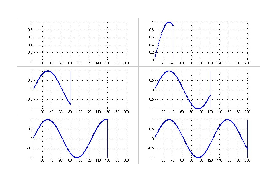
\psfig{file=figures/simple_realtime.eps,width=5.75in}}
  \caption{Simple real-time plot}
  \label{fig:SimpleRealtime}
\end{figure}

\section{Runtime Control and Analysis}
\label{sec:RuntimeControlandAnalysis}

This third revision of the control system application attempts to build on the lessons from previous versions.  This version's centers on two main ideas.  The first is to address the issue of not sharing sensor data, and the second is to expand on the initial success of the ``real-time'' visualizations from the ``TSat Message Center''.  Figure \ref{fig:RuntimeControlDashboard} shows the improvements in the interface over the previous version.  In the lower left are toggles for timers that check the incoming buffer for messages, send requests for sensor data, update the estimator, and update the controller.  Each timer runs on its own loop and can run at different rates.

The top left are the different pages that data gets populate to as the controller runs.  Figure \ref{fig:RuntimeControlDashboard} shows the ``Manual Control'' page that has some manual override controls.

\begin{figure}[H]
  \centerline{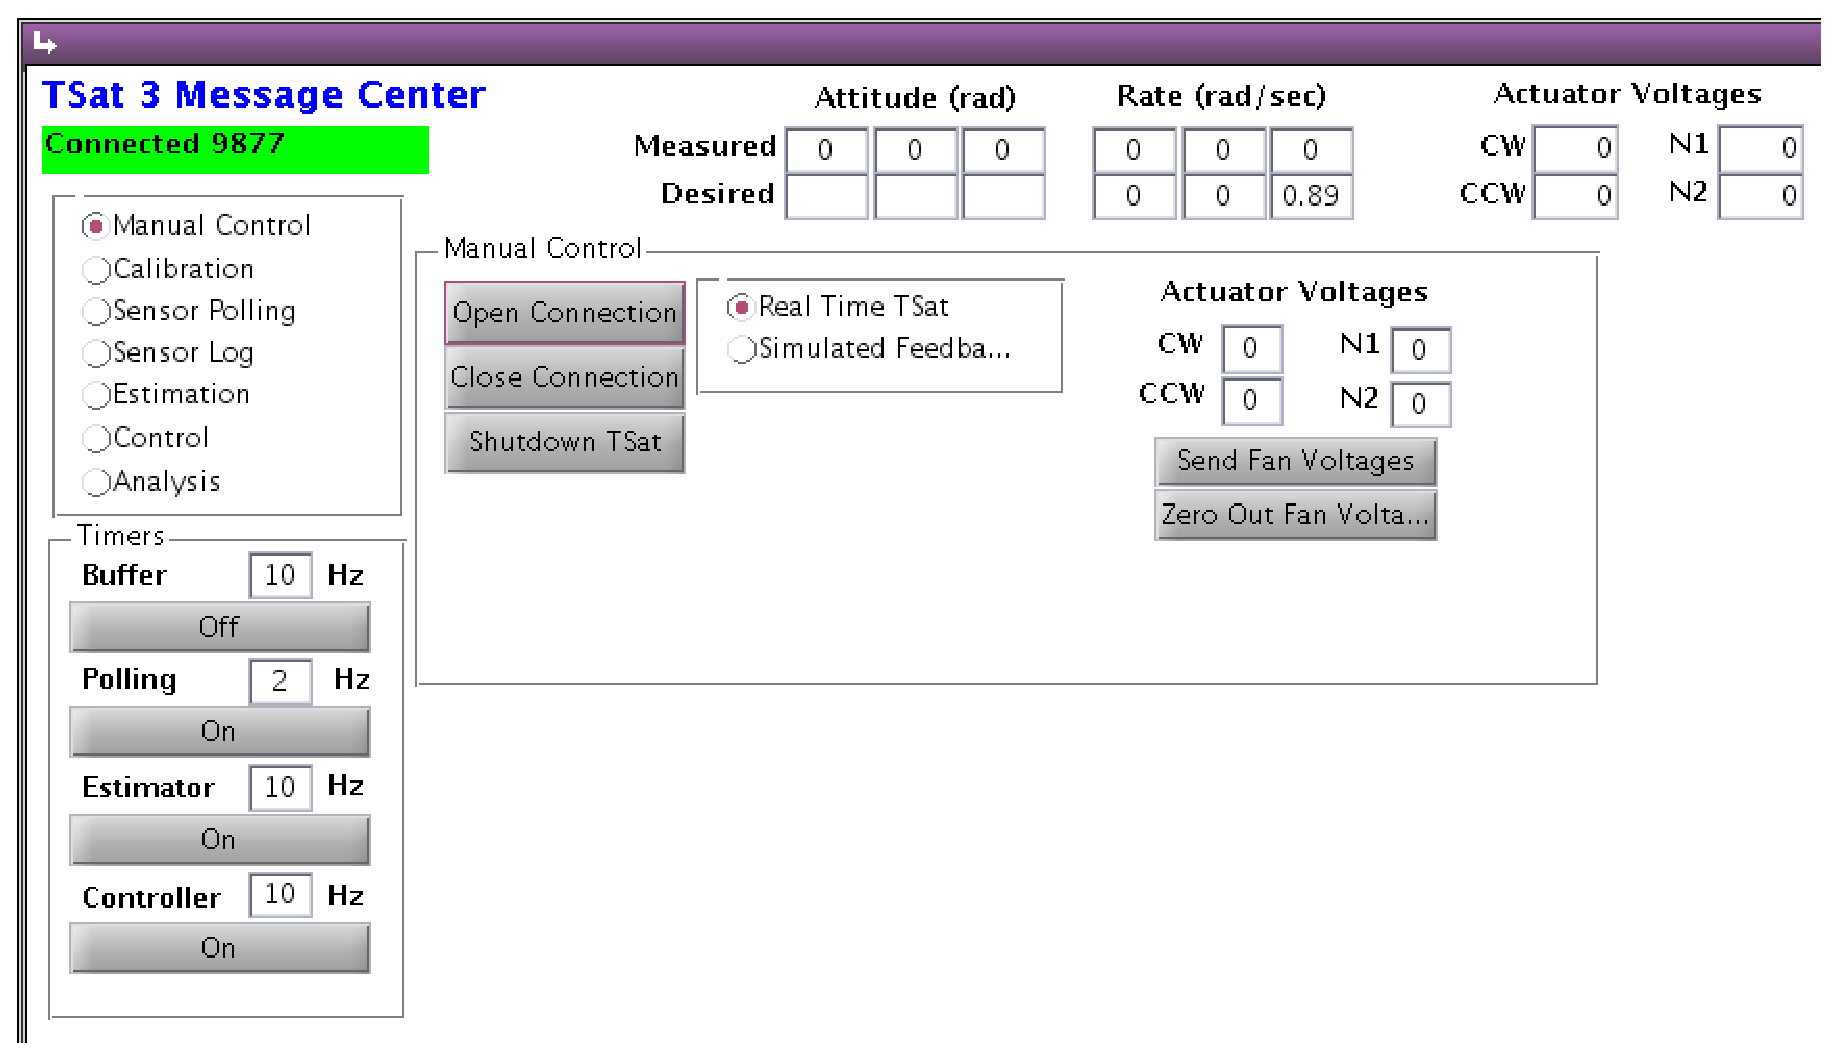
\psfig{file=figures/TSat3MC.eps,width=5.75in}}
  \caption{Runtime Control Dashboard}
  \label{fig:RuntimeControlDashboard}
\end{figure}

Under the ``Sensor Polling'' page, the basic matrix conversion from sensor reading to measured state is visible (Figure \ref{fig:RuntimeStateCalculations}), and as part of the ``Control'' page an early implementation of the SMC controller is visible (Figure \ref{fig:RuntimeSMCVisual}).

\begin{figure}[H]
  \centerline{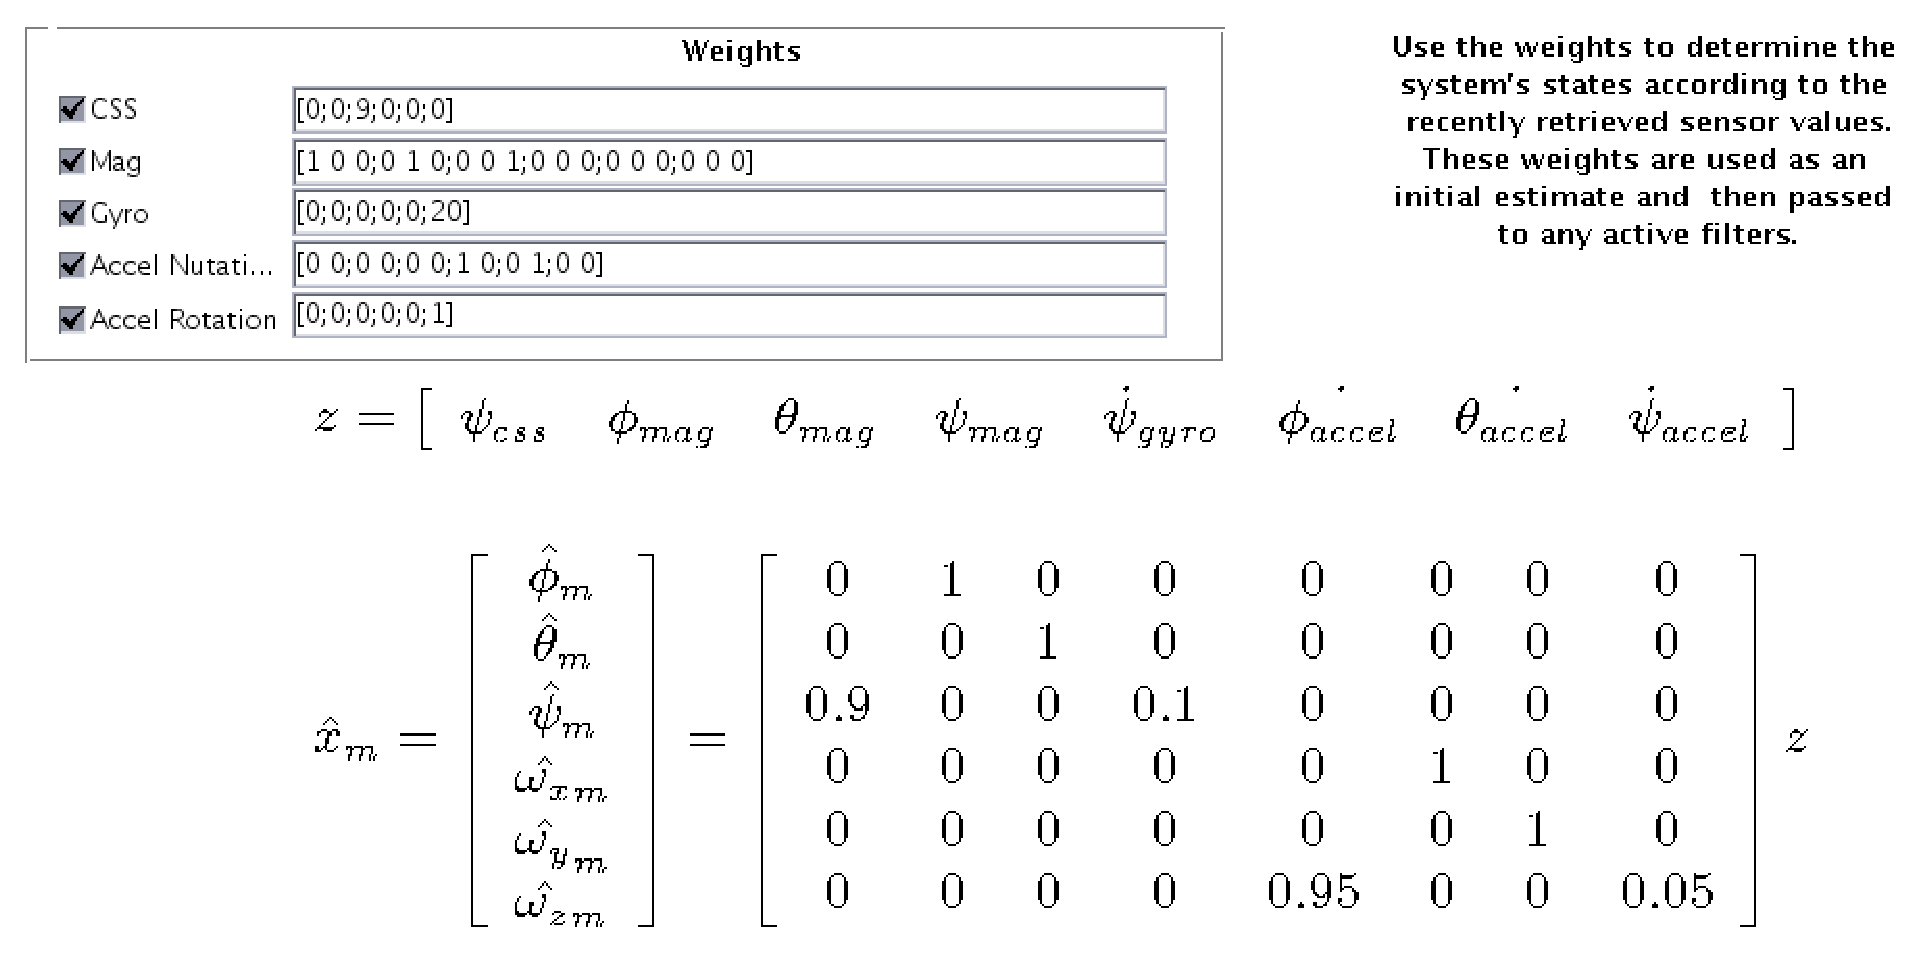
\psfig{file=figures/realtime_ui_formulas.eps,width=5.75in}}
  \caption{Runtime State Calculations}
  \label{fig:RuntimeStateCalculations}
\end{figure}

\begin{figure}[H]
  \centerline{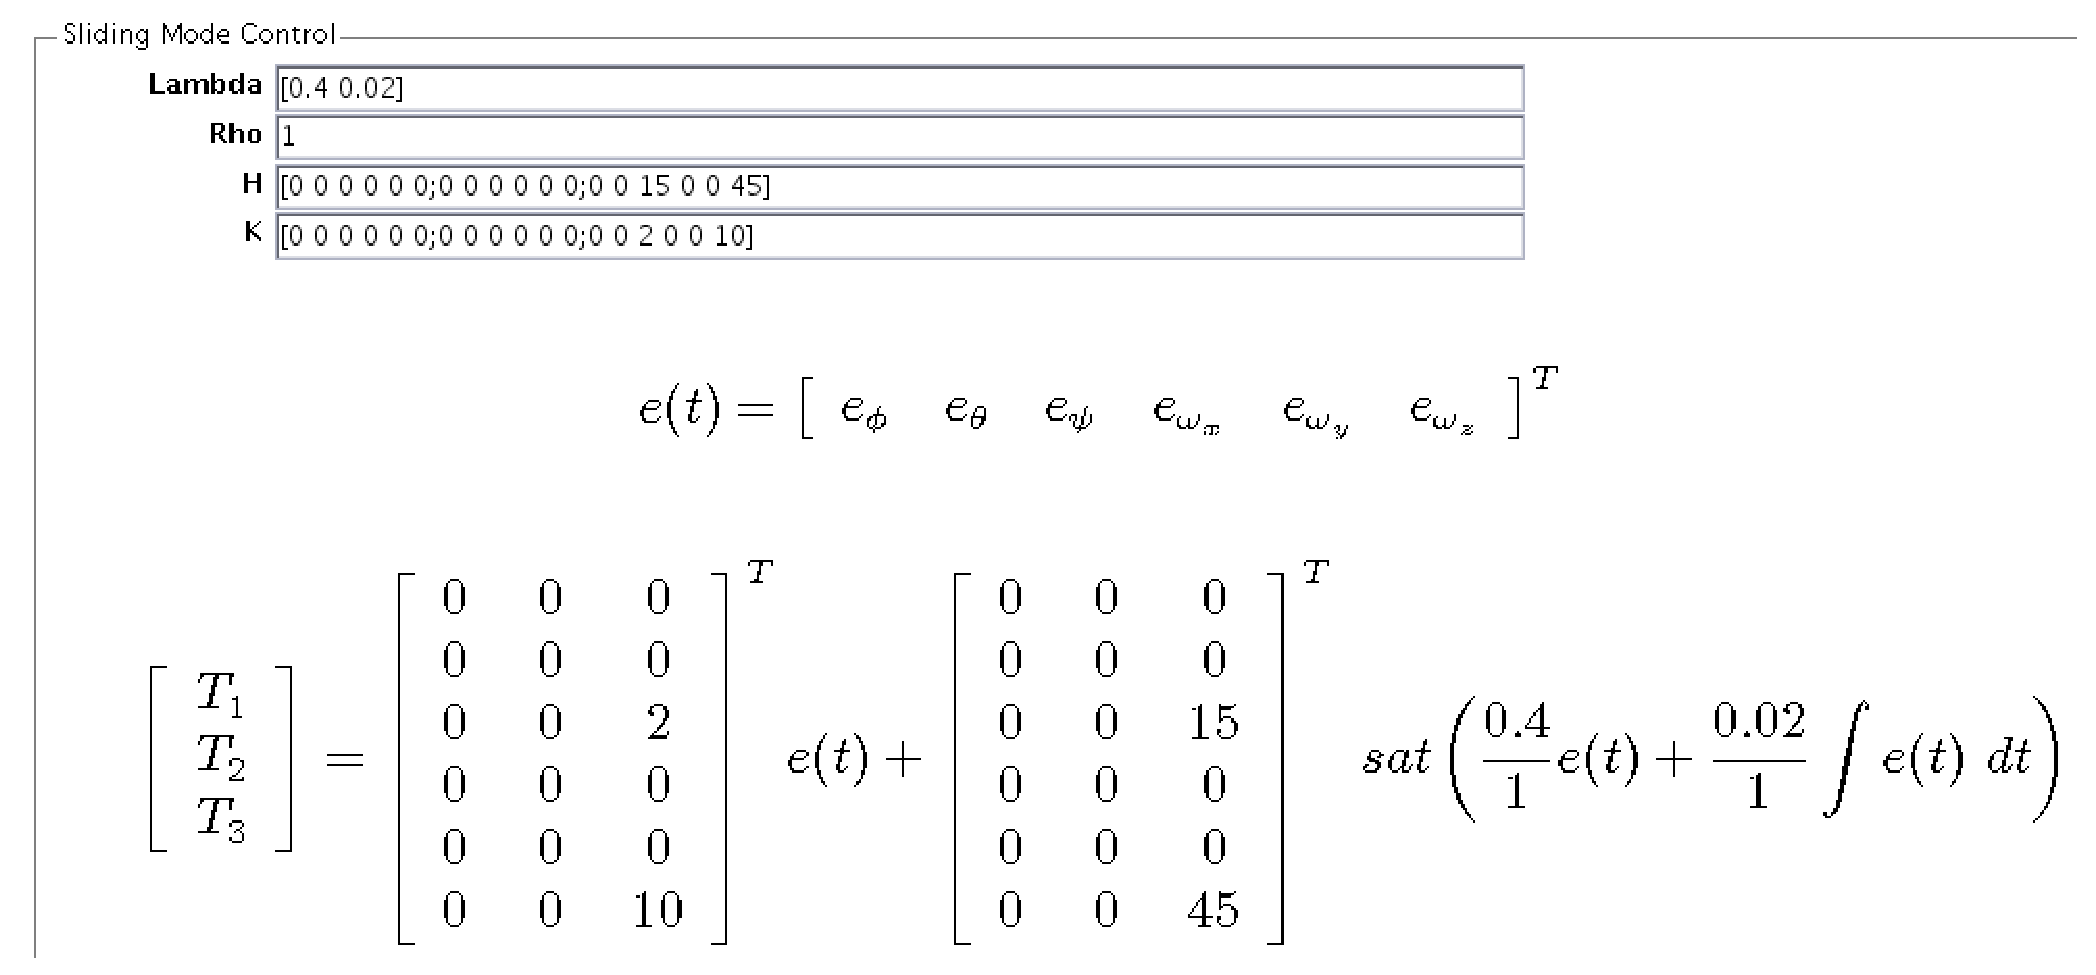
\psfig{file=figures/realtime_ui_smc_update.eps,width=5.75in}}
  \caption{Runtime SMC Visual}
  \label{fig:RuntimeSMCVisual}
\end{figure}

Although visually appealing and including some useful features, this version's main purpose is designed on presenting information and interacting with the user rather than controlling the TableSat.

\section{Object Oriented NSS Control System}
\label{sec:ObjectOrientedNSSControlSystem}

The first three versions of the control system establish a collection of requirements for a usable system.  The control system should:

\begin{itemize}
\item allow access to information as an experiment or simulation runs
\item be fault-tolerant
\item have methods to ensure consistency through improvements
\item allow sensor data to be shared by multiple consumers
\item convey information to the user in an easily consumable format
\item be configured for modular and reusable code
\end{itemize}

The fourth version (Appendix \ref{chap:NSSObjectOrientedSourceCode}) is based on an object oriented architecture written for a Numerical Simulation Software (NSS such as MATLAB or Octave).  An object oriented class is created for a particular concept or data type.  Snippet \ref{code:matlab_oo_base} shows the basic structure of a class of data that represents a system's body-fixed angular velocities (body rates).
\begin{listing}[H]
\begin{singlespace}
  \begin{minted}[mathescape,linenos,numbersep=10pt,frame=lines,framesep=2mm]{matlab}
classdef bodyRate
  properties
    w
  end
  methods
    function self = bodyRate(w)
      self.w = w
    end
  end
end
  \end{minted}
\caption{NSS object oriented base}
\label{code:matlab_oo_base}
\nocite{minted}
\end{singlespace}
\end{listing}
The \verb|bodyRate| class in Snippet \ref{code:matlab_oo_base} contains the property \verb|w|, which stores the body rate values $\omega_x, \omega_y, \text{ and } \omega_z$ that are passed to it on initialization.  Additional methods can then be added to the class in order to perform common operations such as adding two body rates together.  Snippet \ref{code:matlab_oo_base_simple_method} shows the creation of the addition method which is called by the infix operator ``\verb|+|''.
\begin{listing}[H]
\begin{singlespace}
  \begin{minted}[mathescape,linenos,numbersep=10pt,frame=lines,framesep=2mm]{matlab}
classdef bodyRate
  properties
    w
  end
  methods
    function self = bodyRate(w)
      self.w = w
    end
    function self = bodyRate(w)
      self.w = w
    end
    function br = plus(a,b)
      br = bodyRate(a.w + b.w);
    end
  end
end
  \end{minted}
\caption{NSS object oriented simple method}
\label{code:matlab_oo_base_simple_method}
\nocite{minted}
\end{singlespace}
\end{listing}
Now that the object knows how to add itself to another body rate the class can be used as
\begin{listing}[H]
\begin{singlespace}
  \begin{minted}[mathescape,linenos,numbersep=10pt,frame=lines,framesep=2mm]{matlab}
>> br1 = bodyRate([1 3 -4]')
>> br2 = bodyRate([-0.5 -5 3]')
>> br3 = br1 + br2
>> disp(br3.w)
    0.5000
   -2.0000
   -1.0000
  \end{minted}
\caption{Using infix + operator with a custom class definition}
\label{code:add_body_rates}
\nocite{minted}
\end{singlespace}
\end{listing}

The particular example of the \verb|bodyRate| above demonstrates the basic design of a new class, but is ``overkill'' if all that's needed is to sum body rates, which can just be accomplished with matrix algebra.  The object oriented class becomes particularly useful for situations that require a bit more complexity, such as quaternion multiplication.  The first three versions of the software use Euler angles for attitude parametrization.  As quaternions are favored during implementation for numerical stability, this fourth version uses quaternion attitude parametrization.

One common issue with quaternions, is that they are composed from a vector of three parameters and a scalar value ($\bs{q} = q_1 \bs{i} + q_2 \bs{j} + q_3 \bs{k} + q_0$).  To add to the confusion, the scalar quantity is often interchanged, depending upon the preference of the user, between the first and last position of the quaternion tensor.  Therefore, so when represented in the 4x1 vector notation it becomes difficult to determine which format is being used.

As shown in Equation (\ref{eqn:QuaternionMultiplication}), the quaternion multiplication is defined as
\begin{equation}
  \bs{q} = \bs{a} \otimes \bs{b} = \bs{a}_v b_0 + \bs{b}_v a_0 + \bs{a}_v \times \bs{b}_v + a_0 b_0 - \bs{a}_v \cdot \bs{b}_v
\end{equation}
although most references use the matrix notation
\begin{equation}
  \begin{bmatrix} q_1 \\ q_2 \\ q_3 \\ q_0 \end{bmatrix} =
  \begin{bmatrix}
    a_0 & - a_3 &   a_2 & a_1 \\
    a_3 &   a_0 & - a_1 & a_2 \\
  - a_2 &   a_1 &   a_0 & a_3 \\
  - a_1 & - a_2 & - a_3 & a_0
  \end{bmatrix}
  \begin{bmatrix}
  b_1 \\ b_2 \\ b_3 \\ b_0
  \end{bmatrix}
\end{equation}
Using a quaternion class with vector and scalar properties keeps the values separate and distinct.  As such, the class gets augmented to operate with the multiplication infix operator, the user does not need to be concerned with the scalar term placement.

Snippet \ref{code:matlab_quaternion_class} uses a simplified version of the quaternion class where the properties keep the vector and scalar quantities
separated allowing Equation \ref{eqn:QuaternionMultiplication} to be used.
\begin{listing}[H]
\begin{singlespace}
  \begin{minted}[mathescape,linenos,numbersep=10pt,frame=lines,framesep=2mm]{matlab}
classdef quaternion
  properties
    vector
    scalar
  end
  methods
    function self = quaternion(vector, scalar)
      self.vector = vector;
      self.vector = scalar;
    end
    function q = mtimes(a,b)
      av = a.vector;
      bv = b.vector;
      s = a.scalar * b.scalar - (av(1)*bv(1)+av(2)*bv(2)+av(3)*bv(3));
      v = av * b.scalar + bv * a.scalar + cross(av,bv);
      q = quaternion(v, s);
    end
  end
end
  \end{minted}
\caption{Simplified quaternion class}
\label{code:matlab_quaternion_class}
\nocite{minted}
\end{singlespace}
\end{listing}

In order to ensure the consistent functionality of the classes created, this version also incorporates unit tests.  These tests are designed along with the creation of the class.  For the \verb|bodyRate| example, a test can be written to ensure that the sum shown in Snippet \ref{code:add_body_rates} continues to produce the correct result.  This extra effort improves the reliability of the system since if edit are required to support a new use case, the series of existing tests can verify that no preexisting behavior is broken.

An additional class that is very useful is the \verb|tPlot| class.  This class is an extension of the ``real-time'' plots from previous versions.  This class addresses one of the main goals cited in the Chapter \ref{chap:Introduction} of providing state information from both the simulation and experiment as it occurs to give the researcher insight into the system.  This is just not possible through scope outputs or other post processing.

The \verb|tPlot| class creates a plot window and maintains a connection to that plot allowing for any type of information available to be displayed as it occurs.  One of the most useful representations is a wireframe of the TableSat IA.  This ability to represent changes to the physical system as it appears in real life rather than through a series of time series plots after the fact is a powerful tool for control systems engineers.

As the system runs, a quaternion state is updated to represent a new attitude.  As with the multiplication shown in Snippet \ref{code:matlab_quaternion_class}, a method exists that takes a point in 3D space, applies the rotation represented by the quaternion, and returns the transformed point coordinates.  When performed against the set of points that makes up the wireframe TableSat, the update quaternions can update the new locations for the points and pass them through the \verb|tPlot| instance to the 3D representation.  This process is performed to validate truth model motions along with estimator and controller effectiveness compared to the measured or estimated states.

Figure \ref{fig:RuntimeSatelliteVisualization} shows frame captures from the simulation of a quaternion-based attitude controller.  Frames proceed through time from left to right and display the desired state (black), the current state (blue), and the actuator locations (blue circles) along with any force being applied by the actuator.  Through this one visualization, an entire system can be assessed including the the desired system's state propagation, and the ``true'' system's reactions to control inputs, whether the correct thrusters are being actuated and in the correct direction, if the controller provides an adequately stable response, and whether vibrations are likely be to introduced into boom dynamics.

\begin{figure}[ht]
  \centerline{\psfig{file=figures/p-attitude-control-video-tile.eps,width=5.75in}}
  \caption{Runtime Satellite Visualization}
  \label{fig:RuntimeSatelliteVisualization}
\end{figure}

Even with the powerful visualization tool, this version runs into issues related to its NSS environment.  While the class structure is supported and enables the possibility of advanced analyses, handling and diagnosing unforeseen conditions in the code is difficult.  Along with some idiosyncrasies in creating copies of objects or extending them from a handler base class to allow for an object to edit itself, the biggest obstacle and what motivates for the final revision in Chapter \ref{chap:TSatPy} is the difficulty in debugging.  In some uncommon cases the system's state is unstable for no easily apparent reason, and determining the issue proves prohibitively difficult.
